\section{Matched-Accuracy Sparse-Query Workloads}
\label{app:matchedaccuracy}

\paragraph{Question and frozen protocol.}
The comparison asks when evaluating a small set of topological insertion
scores is cheaper than constructing a reusable volumetric primal--adjoint
field. It does not presume that a grid-free method is faster. Before the
measured sweep, we fixed four geometries, query counts $8,32,128,512$, five
random seeds, TWoS path budgets $256,1024,4096$, and longest-axis multigrid
counts $49,65,97,129$. The objects are the existing housing, branching
manifold, annular spreader, and the 69,674-triangle Bunny. All use distinct
compact primal and adjoint sources. The Bunny has sensor center
$(0.15,-0.15,0)$ and radius $0.07$, a primary source centered at
$(-0.15,-0.15,0)$ with radius $0.085$ and amplitude $35$, and sensor heating
with radius $0.06$ and amplitude $4$. Thus this test differs from the earlier
Bunny compliance crossover; it does not retrospectively replace its objective.

A scrambled Sobol pool with seed 17092026 fixes feasible sites without
consulting scores. The last admissible pool point determines a radius-$0.04$
cavity. The 512 query sites avoid this prospective cavity by a center-distance
margin of $0.10$. Both methods evaluate the original domain and the domain
with this fixed cavity. The edit is a controlled workload perturbation, not
an optimized insertion or a claimed improvement in objective value.
Nested batches contain $8,24,96,384$ new sites, giving the stated prefix counts.
Five paired random seeds are $1611,2711,3811,4911,6011$.

\paragraph{Giving the grid its legitimate reuse.}
The multigrid baseline uses the same masked finite-difference operator and
geometric V-cycle as the previous study. Its primal and adjoint share the
geometry hierarchy. The new query backend retains both solved finest-grid
fields, so additional sites on an unchanged domain require only trilinear
interpolation. A cavity insertion invalidates the cached fields; the common
outer-mesh acceleration structure remains available to both methods.
Each method--budget--seed combination has a fresh process, preventing peak
memory from being inherited from another method. We measure mesh setup
separately and cumulative wall time through every prefix, including field
construction where incurred, request handling, and output writing. These
measurements describe this implementation, not an optimized lower bound on
multigrid query latency. All timing runs execute serially on four threads;
method order rotates with seed. Independent reference construction is
excluded from each method's query cost. Cached repeats must reproduce all
primal, adjoint, and score values within eight machine epsilons after CSV
serialization and make no geometry queries. Across 360 repeat checks the
maximum absolute discrepancy is $1.36\times10^{-20}$.

\paragraph{Accuracy and reference gates.}
For a query prefix of size $Q$, let $s^{257}$ denote the score vector from
MG257 and $\widehat s_{m,b,r}$ the tested method $m$, budget $b$, and seed $r$.
We measure
\[
 e_{m,b,r}(Q)=\frac{\|\widehat s_{m,b,r}-s^{257}\|_2}{\|s^{257}\|_2}.
\]
This is reference-relative numerical error, not known continuum error.
In particular, the grid reference and multigrid baseline share a
 discretization family. We therefore report a refinement discrepancy
$\delta_Q=\|s^{193}-s^{257}\|_2/\|s^{257}\|_2$ and an independent
Monte Carlo check at 32 fixed, evenly indexed query sites. Eight independent
8,192-path batches give mean $\bar s$ and componentwise standard errors.
Let $\eta$ be the norm of that standard-error vector divided by the norm of
the grid reference on those sites, and $d$ the similarly normalized
$\|\bar s-s^{257}\|_2$. For a target $\tau$, the declared diagnostic gate is
\[
 \delta_Q\leq\tau/4,\qquad \eta\leq\tau/4,\qquad
 d\leq\tau/4+2\eta.
\]
These gates are diagnostic tolerances, not probabilistic error certificates:
the factor two is not a proved multivariate confidence radius, and the
spot check does not cover every site. Grid convergence alone cannot rule out
shared bias. A zero or nonfinite reference norm is unresolved. The primary
target is $\tau=0.20$; $0.10$ and $0.40$ are predeclared sensitivity targets.
No gate is relaxed after inspecting results.

\paragraph{Uncertainty and selection.}
We resample the five paired seeds 10,000 times with fixed bootstrap seed
20260917, reporting pointwise percentile intervals for mean relative error
and mean time. A budget is eligible only if its upper 97.5th percentile
for mean error is at most $\tau$ and the reference gates pass. We select the
fastest eligible tested budget within each method. Missing eligible budgets
are reported explicitly, never converted to infinite speedups. Intervals
for selected runtime ratios resample paired seeds jointly; they are
descriptive after selection and are not simultaneous or selection-adjusted
confidence statements. Timing and sampling variation do not enclose
termination, floating-point, geometric, or discretization bias. All tested
budgets, reference diagnostics, and unsuccessful targets accompany the paper.

\paragraph{Measured results.}
Table~\ref{tab:matched-primary} reports the predeclared 20\% target. A dash means an unresolved reference or no eligible tested budget; it never denotes an infinite speedup. The analytic-source and incremental-grid extensions were introduced after the first housing result and frozen before their own measurements. Their results are therefore separate diagnostic extensions, not retroactively part of the initial protocol.
\begin{table}[t]\centering\small
\caption{Calibration results at the 20\% reference-relative accuracy target. Times include every batch through the listed query count. MG is the fastest eligible tested resolution and reuse variant. RB denotes exact-source integration in ideal arithmetic. All quantities are empirical; source restrictions and numerical-reference gates apply.}
\label{tab:matched-primary}
\begin{tabular}{llrrrrrr}\toprule
Object & State & Queries & TWoS (s) & TWoS--RB (s) & MG (s) & MG/RB & RB paths\\\midrule
Branch & edited & 8 & 0.997 & 0.823 & 0.049 & 0.06 & 4096\\
Branch & edited & 512 & 53.502 & 13.063 & 0.053 & 0.00 & 1024\\
Branch & original & 8 & 0.982 & 0.877 & 0.090 & 0.10 & 4096\\
Branch & original & 512 & 49.404 & 11.476 & 0.095 & 0.01 & 1024\\
Bunny & edited & 8 & 1.635 & 0.409 & 0.122 & 0.30 & 1024\\
Bunny & edited & 512 & 77.790 & 17.474 & 0.128 & 0.01 & 1024\\
Bunny & original & 8 & 1.406 & 0.322 & 0.201 & 0.62 & 1024\\
Bunny & original & 512 & 71.133 & 18.535 & 0.208 & 0.01 & 1024\\
Bunny compliance & edited & 8 & -- & 0.023 & 0.073 & 3.17 & 64\\
Bunny compliance & edited & 512 & -- & 4.372 & 0.079 & 0.02 & 256\\
Bunny compliance & original & 8 & -- & 0.028 & 0.116 & 4.19 & 64\\
Bunny compliance & original & 512 & -- & 4.430 & 0.120 & 0.03 & 256\\
Housing & edited & 8 & -- & 0.084 & 0.031 & 0.37 & 1024\\
Housing & edited & 512 & 22.283 & 4.875 & 0.036 & 0.01 & 1024\\
Housing & original & 8 & -- & 0.084 & 0.085 & 1.02 & 1024\\
Housing & original & 512 & 21.718 & 4.595 & 0.089 & 0.02 & 1024\\
Ring & edited & 8 & -- & 0.255 & 0.039 & 0.15 & 1024\\
Ring & edited & 512 & 54.190 & 11.832 & 0.043 & 0.00 & 1024\\
Ring & original & 8 & -- & 0.239 & 0.102 & 0.43 & 1024\\
Ring & original & 512 & 49.844 & 12.061 & 0.109 & 0.01 & 1024\\
\bottomrule\end{tabular}\end{table}
\begin{table}[t]\centering\small
\caption{Independent reference diagnostics. Refinement discrepancies are shown at 8 and 512 sites; the 32-site Monte Carlo diagnostic is common to each state. Values are percentages. These quantities are not rigorous error bounds.}
\begin{tabular}{llrrrr}\toprule Object & State & $\delta_8$ & $\delta_{512}$ & MC SE norm & MC--grid discrepancy\\\midrule
Branch & edited & 1.34 & 1.29 & 3.07 & 5.37\\
Branch & original & 1.34 & 1.29 & 3.35 & 5.62\\
Bunny & edited & 0.84 & 0.74 & 3.79 & 2.45\\
Bunny & original & 0.84 & 0.74 & 3.86 & 2.64\\
Bunny compliance & edited & 1.16 & 1.27 & 0.57 & 2.49\\
Bunny compliance & original & 1.16 & 1.27 & 0.56 & 2.44\\
Housing & edited & 0.70 & 3.03 & 2.87 & 6.11\\
Housing & original & 0.70 & 3.03 & 2.87 & 6.11\\
Ring & edited & 1.36 & 1.03 & 2.98 & 7.01\\
Ring & original & 1.36 & 1.03 & 2.98 & 7.01\\
\bottomrule\end{tabular}\end{table}
\begin{figure}[p]\centering
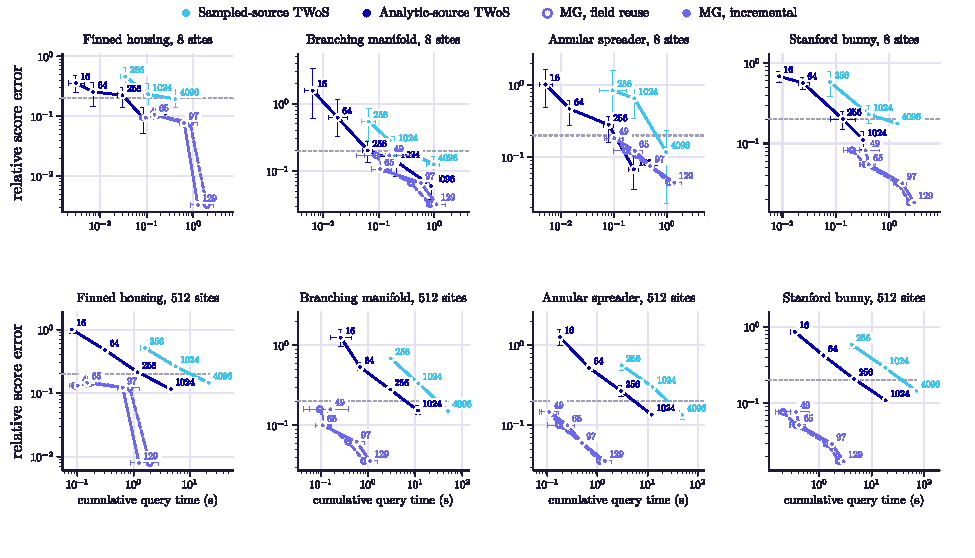
\includegraphics[width=\textwidth]{figures/matched-accuracy-original.pdf}
\caption{All measured budgets on the original domain, at 8 sites (top) and 512 sites (bottom). Bars are pointwise 95\% bootstrap intervals over five seeds; they exclude numerical-reference bias. Dashed horizontal lines mark the 20\% target before applying the independent reference gates. Numbers label path counts or longest-axis grid counts. Original and source-integrated TWoS and both grid reuse variants are retained.}\end{figure}
\begin{figure}[p]\centering
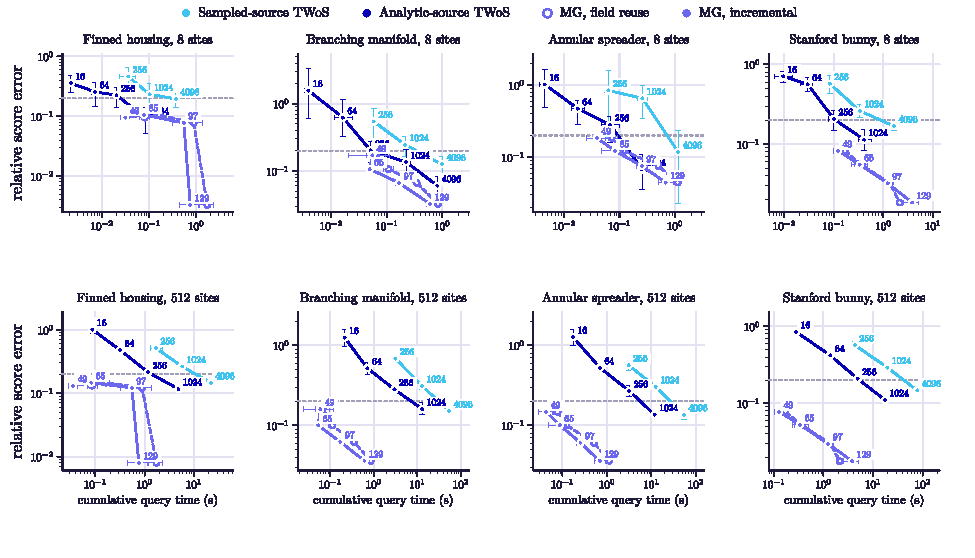
\includegraphics[width=\textwidth]{figures/matched-accuracy-edited.pdf}
\caption{All measured budgets on the edited domain, at 8 sites (top) and 512 sites (bottom). Bars are pointwise 95\% bootstrap intervals over five seeds; they exclude numerical-reference bias. Dashed horizontal lines mark the 20\% target before applying the independent reference gates. Numbers label path counts or longest-axis grid counts. Original and source-integrated TWoS and both grid reuse variants are retained.}\end{figure}
\begin{figure}[p]\centering
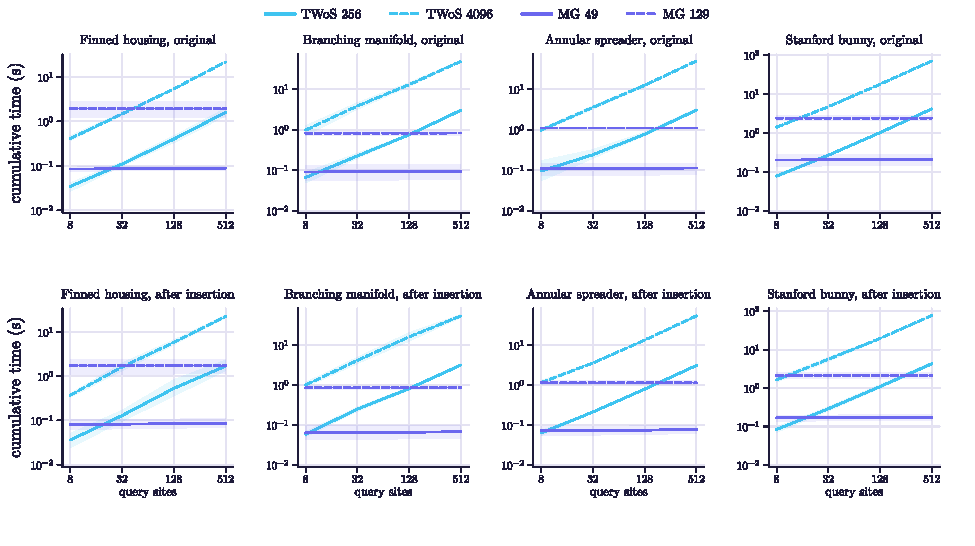
\includegraphics[width=\textwidth]{figures/matched-accuracy-scaling.pdf}
\caption{Measured query-count scaling at fixed budgets in the initially frozen sweep. Shaded bands show pointwise 95\% bootstrap intervals for mean time. Original-source TWoS scales with the number of sites, whereas solved-field multigrid amortizes its setup. These fixed-budget curves do not assert matched accuracy.}\end{figure}
\paragraph{Fresh-seed confirmation and its failures.}
The four apparent 20\%-target wins selected from calibration did not pass both fresh-seed rules. The three compliance cases exceeded the mean-error upper-endpoint threshold; the housing timing interval included no advantage. We then declared a separate, fixed 256-path follow-up for both eight-site compliance states, with 20 further fresh seeds and no subsequent budget search. All results are retained below. These pointwise bootstrap checks are not simultaneous confidence guarantees.
\begin{table}[t]\centering\small
\caption{Fresh-seed query confirmations. Times exclude common geometry loading. Error upper endpoints and speed intervals use 10,000 paired bootstrap resamples of 20 seeds. Passing requires error upper endpoint $\leq20\%$ and speed-ratio lower endpoint $>1$. Every row uses MG49.}
\setlength{\tabcolsep}{3.2pt}
\begin{tabular}{llrrrrrr}\toprule Workload / state & Stage & Sites & Paths & TWoS / MG (ms) & Error upper & MG/TWoS interval & Pass\\\midrule
Bunny compliance / edited & Selected & 8 & 64 & 23.3 / 78.4 & 21.8\% & [2.51, 4.57] & no\\
Bunny compliance / original & Selected & 8 & 64 & 28.7 / 341.3 & 21.3\% & [6.21, 19.36] & no\\
Bunny compliance / original & Selected & 32 & 64 & 74.0 / 136.8 & 20.8\% & [1.58, 2.13] & no\\
Housing / original & Selected & 8 & 1024 & 137.4 / 131.9 & 13.6\% & [0.58, 1.54] & no\\
Bunny compliance / edited & Fixed 256 & 8 & 256 & 83.1 / 72.8 & 10.3\% & [0.69, 1.11] & no\\
Bunny compliance / original & Fixed 256 & 8 & 256 & 89.9 / 113.9 & 10.2\% & [1.05, 1.50] & yes\\
\bottomrule\end{tabular}\end{table}


\paragraph{Random-stream indexing audit and correction.}
The retained legacy implementation XORs hashes of a seed, site index, and
walk index. When a driver seed equals a walk-index offset, this construction
can cancel or swap identifiers and reuse a stream across nominal repetitions.
For the present five seeds and four query batches, this affects twelve
indices at the 4,096-path budget; budgets through 1,024, the high-seed
reference batches, and the fresh holdout seeds do not have that structural
overlap. We correct the affected calibration draws, retain the superseded
outputs, and enumerate the resulting stream keys to check uniqueness.
This is a disclosed correctness amendment, not a selection based on outcomes.

Let $I$ be the fixed set of affected indices. We replay their original
paths and replacement paths with unused indices, obtaining $(U_i,P_i)$ and
$(U'_i,P'_i)$. The corrected sufficient statistics are
\[
 S'_U=N\bar U+\sum_{i\in I}(U'_i-U_i),\qquad
 S'_P=N\bar P+\sum_{i\in I}(P'_i-P_i),
\]
\[
 S'_{UP}=\sum_i U_iP_i+
       \sum_{i\in I}(U'_iP'_i-U_iP_i),\qquad
 \widehat S'=\frac{S'_US'_P-S'_{UP}}{N(N-1)}.
\]
To verify the reconstruction, split each original sum into indices inside
and outside $I$: subtraction removes exactly the old inside terms, and
addition supplies exactly their replacements. Thus these are precisely the
sums of the corrected $N$ pairs in exact arithmetic. Selection of $I$ depends
only on stream identities, so it does not condition on observed path values.
Under the ideal independent-stream model, unique keys give the intended
independent pairs and the usual off-diagonal-product proof applies. Distinct
PRNG keys alone are not a mathematical proof of PRNG independence.
We check floating-point reconstruction against complete clean runs on each
affected workload; all replay work is charged to corrected query costs.

\paragraph{Fresh-seed confirmation of apparent speed wins.}
Budgets selected from five calibration seeds are not independently validated
by those same seeds. Before measuring the extensions, we therefore fix a
confirmation protocol: every apparent 20\%-target speed win retains its
selected configurations and uses 20 fresh seeds, alternating method order.
The upper bootstrap mean-error endpoint must remain below 20\%, and the
lower paired runtime-ratio endpoint must exceed one, to call the result a
confirmed win. Failed confirmations remain reported. The same numerical
reference gates apply; these pointwise checks are neither simultaneous tests
nor continuum-error certificates. Offline tuning and reference construction
are excluded from query costs, so this comparison is not an online accuracy
controller.
